\taskpic{Определите сопротивление полубесконечной цепочки между точками
  $A$ и $B$, если сопротивление каждого звена равно $R$.}{
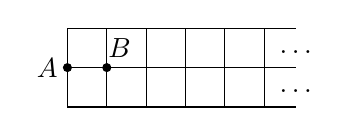
\begin{tikzpicture}
  \draw[step=0.5] (0,0) grid (2.9,1);
  \draw[fill=black] (0,0.5) circle (0.05) node[left] {$A$};
  \draw[fill=black] (0.5,0.5) circle (0.05) node[above=7,right=-3]
  {$B$};
  \draw (2.9,0.2) node {$\ldots$};
  \draw (2.9,0.7) node {$\ldots$};
\end{tikzpicture}
}